\documentclass[aspectratio=169]{beamer}

\usepackage{spbgeu-beamer}
\usepackage[russian]{babel}
\usepackage{fix-cm}
\usepackage{amsmath,amssymb,mathtools}
\usepackage{booktabs,array,tabularx,multirow}
\usepackage{pgfplots}
\usepackage{bm}
\usefonttheme[onlymath]{serif}
\usetikzlibrary{arrows.meta,positioning,fit,decorations.pathreplacing}
\pgfplotsset{compat=1.18}

\DeclareMathOperator{\sgn}{sgn}

\newcommand{\Body}{\fontsize{21}{27}\selectfont}
\newcommand{\SmallBody}{\fontsize{21}{27}\selectfont}
\newcommand{\TinyBody}{\fontsize{21}{27}\selectfont}
\newcommand{\FormulaBody}{\fontsize{21}{27}\selectfont}
\newcommand{\SplitBody}{\fontsize{18}{23}\selectfont}
\newcommand{\DisplayFormula}[1]{%
  \[
    #1
  \]
}
\newcommand{\CenteredDisplayFormula}[1]{%
  \par\begingroup
    \leftskip=0pt%
    \rightskip=0pt%
    \parfillskip=0pt%
    \noindent\makebox[\linewidth][c]{%
      \(\displaystyle\begin{gathered}#1\end{gathered}\)%
    }%
  \par\endgroup
}

\newcommand{\Accent}[1]{{\color{spbgeuTeal}\bfseries #1}}
\newcommand{\Purple}[1]{{\color{spbgeuPurple}\bfseries #1}}
\newcommand{\Muted}[1]{{\color{spbgeuText!70}#1}}

\newcommand{\ReportSvmMargin}{%
\resizebox{.99\linewidth}{!}{%
\begin{tikzpicture}[scale=1.20, >=Latex, every node/.style={font=\small}]
    \draw[->, gray!70] (-4.5,0) -- (4.7,0) node[right] {$x_1$};
    \draw[->, gray!70] (0,-3.0) -- (0,3.1) node[above] {$x_2$};

    \filldraw[fill=blue!12, draw=blue!70, thick, fill opacity=0.45]
        (-3.65,1.00) -- (-2.65,1.75) -- (-0.72,1.00) -- (-1.28,-1.00) -- (-3.30,-1.55) -- cycle;
    \filldraw[fill=red!12, draw=red!70, thick, fill opacity=0.45]
        (0.72,-1.00) -- (1.28,1.00) -- (3.15,1.55) -- (3.80,-0.15) -- (3.00,-1.60) -- cycle;

    \foreach \x/\y in {-3.65/1.00,-2.65/1.75,-0.72/1.00,-1.28/-1.00,-3.30/-1.55}
        \fill[blue!65] (\x,\y) circle (2.4pt);
    \foreach \x/\y in {-3.05/0.85,-2.75/-0.65,-2.35/0.35,-2.45/-1.15,-1.75/0.55,-1.65/-0.35}
        \fill[blue!65] (\x,\y) circle (2.1pt);
    \foreach \x/\y in {0.72/-1.00,1.28/1.00,3.15/1.55,3.80/-0.15,3.00/-1.60}
        \fill[red!70] (\x,\y) circle (2.4pt);
    \foreach \x/\y in {1.65/0.45,2.35/1.05,2.95/0.55,2.15/-0.55,3.20/-0.85,2.55/-1.20}
        \fill[red!70] (\x,\y) circle (2.1pt);

    \draw[very thick] (-0.8,-2.7) -- (0.8,2.7) node[above] {$L_0$};
    \draw[dashed, thick] (-1.8,-2.7) -- (-0.2,2.7) node[above] {$L_1$};
    \draw[dashed, thick] (0.2,-2.7) -- (1.8,2.7) node[above] {$L_2$};

    \draw[->, thick] (0,0) -- (-1.2,0.36) node[above left, fill=white, inner sep=1pt] {$w$};
    \draw[thin, gray!75, line cap=round] (-0.20,0.06) -- (-0.29,-0.24) -- (-0.09,-0.30);
    \draw[<->, gray!75] (-1.17,-0.57) -- (0.67,-1.12)
        node[midway, below=4pt, fill=white, inner sep=1pt, text=black] {$h=\frac{2}{\|w\|}$};

    \node[blue!65] at (-3.25,2.1) {$\xi=+1$};
    \node[red!70] at (3.15,2.1) {$\xi=-1$};
\end{tikzpicture}}%
}

\newcommand{\ReportSvmSupportVectors}{%
\resizebox{.84\linewidth}{!}{%
\begin{tikzpicture}[scale=1.08, >=Latex, every node/.style={font=\small}]
    \draw[very thick] (-0.6,-2.5) -- (0.7,2.5) node[above] {$L_0$};
    \draw[dashed, thick] (-1.7,-2.5) -- (-0.4,2.5) node[above left] {$L_1$};
    \draw[dashed, thick] (0.5,-2.5) -- (1.8,2.5) node[above right] {$L_2$};

    \filldraw[fill=blue!12, draw=blue!70, thick, fill opacity=0.45]
        (-3.4,0.1) -- (-2.9,-1.2) -- (-1.36,-1.2) -- (-0.93,0.45) -- (-2.3,1.8) -- (-3.0,1.2) -- cycle;
    \filldraw[fill=red!12, draw=red!70, thick, fill opacity=0.45]
        (0.98,-0.65) -- (2.8,-1.4) -- (3.15,-0.85) -- (3.4,-0.2) -- (3.1,1.1) -- (2.4,1.9) -- (1.29,0.55) -- cycle;

    \foreach \x/\y in {-3.0/1.2,-3.4/0.1,-2.9/-1.2,-2.3/1.8,-2.4/-0.5,-3.05/0.55,-2.75/1.2,-2.55/0.35,-2.25/-0.15,-2.05/1.05,-3.15/-0.55}
        \fill[blue!65] (\x,\y) circle (2.1pt);
    \foreach \x/\y in {3.1/1.1,3.4/-0.2,2.8/-1.4,2.4/1.9,2.3/-0.7,2.75/0.75,2.95/0.2,2.55/-0.45,2.25/1.2,3.15/-0.85,2.6/1.55}
        \fill[red!70] (\x,\y) circle (2.1pt);

    \foreach \x/\y in {-1.36/-1.2,-0.93/0.45}
        \draw[blue!80, very thick] (\x,\y) circle (6pt);
    \foreach \x/\y in {0.98/-0.65,1.29/0.55}
        \draw[red!80, very thick] (\x,\y) circle (6pt);

    \node[align=center] at (0,-3.0) {$\alpha_j>0$};
\end{tikzpicture}}%
}

\newcommand{\ReportSoftMargin}{%
\resizebox{.88\linewidth}{!}{%
\begin{tikzpicture}[
    >=Latex,
    every node/.style={font=\small},
    bluepoint/.style={blue!65, fill=blue!65},
    redpoint/.style={red!70, fill=red!70}
]
    \begin{scope}[rotate=10]
        \draw[dashed, thick, gray!70] (-4.9,1.15) -- (4.9,1.15) node[right, black] {$L_1:\ +1$};
        \draw[very thick] (-4.9,0) -- (4.9,0) node[right] {$L_0$};
        \draw[dashed, thick, gray!70] (-4.9,-1.15) -- (4.9,-1.15) node[right, black] {$L_2:\ -1$};

        \draw[<->, gray!70, thick] (-5.25,-1.15) -- (-5.25,1.15) node[midway, left, black] {$\frac{2}{\|w\|}$};
        \draw[->, thick] (-4.2,0.08) -- (-4.2,1.52) node[above] {$w$};

        \foreach \x/\y in {-4.0/1.62,-3.05/1.43,-1.95/1.59,2.25/1.45,3.25/1.65,4.05/1.47}
            \fill[bluepoint] (\x,\y) circle (2.6pt);
        \foreach \x/\y in {-3.95/-1.59,-2.95/-1.42,-1.85/-1.57,2.15/-1.43,3.10/-1.62,3.95/-1.45}
            \fill[redpoint] (\x,\y) circle (2.6pt);

        \coordinate (BlueV) at (-1.65,0.28);
        \fill[bluepoint] (BlueV) circle (2.9pt);
        \draw[blue!75, very thick] (BlueV) circle (6pt);
        \draw[<->, very thick, blue!75] (-1.65,0.34) -- (-1.65,1.15)
            node[midway, right, xshift=4pt, black, fill=gray!10, inner sep=1pt] {$0<\eta_j<1$};

        \coordinate (RedErr) at (1.1,0.30);
        \fill[redpoint] (RedErr) circle (2.9pt);
        \draw[red!75, very thick] (RedErr) circle (6pt);
        \draw[<->, very thick, red!75] (1.1,0.24) -- (1.1,-1.15)
            node[midway, right, xshift=4pt, black, fill=gray!10, inner sep=1pt] {$\eta_j>1$};
    \end{scope}
    \node[blue!70] at (-3.4,2.05) {класс $+1$};
    \node[red!70] at (3.35,-2.05) {класс $-1$};
\end{tikzpicture}}%
}

\newcommand{\ReportMdmHulls}{%
\resizebox{.72\linewidth}{!}{%
\begin{tikzpicture}[>=Latex, every node/.style={font=\small}]
    \coordinate (A1) at (-3.8,1.1);
    \coordinate (A2) at (-2.4,2.0);
    \coordinate (A3) at (-1.3,0.7);
    \coordinate (A4) at (-1.8,-1.1);
    \coordinate (A5) at (-3.4,-1.4);
    \coordinate (B1) at (1.5,1.2);
    \coordinate (B2) at (3.5,1.7);
    \coordinate (B3) at (4.0,-0.4);
    \coordinate (B4) at (2.6,-1.7);
    \coordinate (B5) at (1.2,-0.7);
    \fill[blue!12] (A1) -- (A2) -- (A3) -- (A4) -- (A5) -- cycle;
    \draw[blue!70, very thick] (A1) -- (A2) -- (A3) -- (A4) -- (A5) -- cycle;
    \fill[red!12] (B1) -- (B2) -- (B3) -- (B4) -- (B5) -- cycle;
    \draw[red!70, very thick] (B1) -- (B2) -- (B3) -- (B4) -- (B5) -- cycle;
    \foreach \p in {A1,A2,A3,A4,A5} \fill[blue!65] (\p) circle (2.4pt);
    \foreach \p in {B1,B2,B3,B4,B5} \fill[red!70] (\p) circle (2.4pt);
    \foreach \x/\y in {-3.0/0.4,-2.6/0.95,-2.25/-0.2,-2.95/-0.75} \fill[blue!65] (\x,\y) circle (2.1pt);
    \foreach \x/\y in {2.0/0.35,2.55/0.85,3.05/-0.25,2.35/-0.9} \fill[red!70] (\x,\y) circle (2.1pt);
    \coordinate (Wone) at (-1.45,0.15);
    \coordinate (Wtwo) at (1.35,0.05);
    \draw[very thick, ->] (Wtwo) -- (Wone) node[midway, above] {$w_1^*-w_2^*$};
    \fill[black] (Wone) circle (2.8pt) node[below left] {$w_1^*$};
    \fill[black] (Wtwo) circle (2.8pt) node[below right] {$w_2^*$};
    \node[blue!70] at (-3.2,2.25) {$C_1$};
    \node[red!70] at (3.4,2.1) {$C_2$};
\end{tikzpicture}}%
}

\newcommand{\ReportMdmStep}{%
\resizebox{.96\linewidth}{!}{%
\begin{tikzpicture}[>=Latex, every node/.style={font=\small}]
    \coordinate (A1) at (-4.55,-0.10);
    \coordinate (A2) at (-3.55,1.55);
    \coordinate (A3) at (-1.70,2.00);
    \coordinate (A4) at (0.45,0.45);
    \coordinate (A5) at (-0.10,-1.15);
    \coordinate (A6) at (-1.65,-1.95);
    \coordinate (A7) at (-3.55,-1.55);
    \coordinate (B1) at (3.10,1.40);
    \coordinate (B2) at (4.95,2.05);
    \coordinate (B3) at (6.35,1.00);
    \coordinate (B4) at (6.95,-0.85);
    \coordinate (B5) at (5.95,-2.00);
    \coordinate (B6) at (4.10,-1.65);
    \coordinate (B7) at (2.85,-0.35);
    \fill[blue!5] (A1)--(A2)--(A3)--(A4)--(A5)--(A6)--(A7)--cycle;
    \draw[blue!70, thick] (A1)--(A2)--(A3)--(A4)--(A5)--(A6)--(A7)--cycle;
    \fill[red!5] (B1)--(B2)--(B3)--(B4)--(B5)--(B6)--(B7)--cycle;
    \draw[red!70, thick] (B1)--(B2)--(B3)--(B4)--(B5)--(B6)--(B7)--cycle;
    \foreach \x/\y in {-3.90/0.20,-3.20/1.00,-2.45/1.35,-2.10/0.10,-2.15/-1.10,-1.25/0.90,-2.85/-1.20} \fill[blue!75] (\x,\y) circle (2pt);
    \foreach \x/\y in {3.70/0.95,4.65/1.15,5.25/0.25,5.80/-0.65,4.25/-0.95,6.00/0.10,4.85/-1.35} \fill[red!75] (\x,\y) circle (2pt);
    \coordinate (Pfrom) at (A1);
    \coordinate (Pto) at (A4);
    \coordinate (X) at (-2.70,-0.90);
    \coordinate (Xnew) at (-1.20,-0.735);
    \coordinate (Y) at (4.95,-0.90);
    \node[blue!80] at (-2.25,2.45) {\Large $C_1$};
    \node[red!80] at (5.00,2.45) {\Large $C_2$};
    \fill[blue!90] (Pfrom) circle (3pt);
    \fill[blue!90] (Pto) circle (3pt);
    \node[left=5pt] at (Pfrom) {$p_k'$};
    \node[right=5pt] at (Pto) {$p_k''$};
    \draw[blue!85, dashed, very thick, ->] (Pfrom) -- (Pto);
    \fill[black] (X) circle (2.5pt);
    \fill[black] (Xnew) circle (2.5pt);
    \node[left=6pt] at (X) {$x_k$};
    \node[below=5pt] at (Xnew) {$x_{k+1}$};
    \draw[black, very thick, ->] (X) -- (Xnew);
    \fill[black] (Y) circle (2.5pt);
    \node[right=6pt] at (Y) {$y_k$};
    \draw[gray!70, dashed, thick] (X) -- (Y) node[pos=0.57, below=5pt] {$w_k$};
    \draw[black, thick] (Xnew) -- (Y) node[pos=0.53, above=5pt] {$w_{k+1}$};
\end{tikzpicture}}%
}

\newcommand{\ReportMdmBridge}{%
\resizebox{.72\linewidth}{!}{%
\begin{tikzpicture}[>=Latex, every node/.style={font=\small}]
    \coordinate (A) at (-1.20,0);
    \coordinate (B) at (1.20,0);
    \coordinate (C) at ($(A)!0.5!(B)$);
    \draw[blue!65, thick] (-4.0,1.05) -- (-2.75,1.50) -- (A) -- (-2.00,-1.30) -- (-3.60,-1.10) -- cycle;
    \draw[red!55, thick] (B) -- (2.25,1.22) -- (3.65,0.96) -- (3.88,-0.74) -- (2.35,-1.18) -- cycle;
    \foreach \x/\y in {-3.55/0.72,-2.75/1.10,-2.05/0.22,-2.35/-0.72,-3.10/-0.65} \fill[blue!65] (\x,\y) circle (2.2pt);
    \foreach \x/\y in {1.95/0.72,2.85/0.88,3.50/0.24,2.90/-0.76,2.00/-0.42} \fill[red!60] (\x,\y) circle (2.2pt);
    \draw[very thick] (A) -- (B);
    \draw[->, thick] ($(B)+(0,0.28)$) -- ($(A)+(0,0.28)$) node[pos=0.65, above=2pt, fill=white, inner sep=1pt] {$v$};
    \fill[black] (A) circle (2.7pt) node[below left=10pt, yshift=10pt, fill=blue!9, inner sep=1pt, font=\scriptsize] {$w_1^*$};
    \fill[black] (B) circle (2.7pt) node[below right=10pt, yshift=10pt, fill=red!8, inner sep=1pt, font=\scriptsize] {$w_2^*$};
    \fill[black] (C) circle (2.2pt) node[right=5pt, fill=white, inner sep=1pt] {$c^*$};
    \draw[very thick] ($(C)+(0,-1.75)$) -- ($(C)+(0,1.75)$);
    \draw[dashed, thick, gray!70] ($(A)+(0,-1.65)$) -- ($(A)+(0,1.65)$) node[pos=0.88, left=4pt, black] {$L_1$};
    \draw[dashed, thick, gray!70] ($(B)+(0,-1.65)$) -- ($(B)+(0,1.65)$) node[pos=0.88, right=4pt, black] {$L_2$};
\end{tikzpicture}}%
}

\newcommand{\ReportGroupStep}{%
\resizebox{.88\linewidth}{!}{%
\begin{tikzpicture}[>=Latex, x=1.25cm, y=1.25cm, every node/.style={font=\normalsize}, line cap=round, line join=round]
    \path[use as bounding box] (-0.2,-2.0) rectangle (8.7,3.5);
    \coordinate (H1) at (1.15,-1.25);
    \coordinate (H2) at (0.95,1.35);
    \coordinate (H3) at (2.65,2.35);
    \coordinate (H4) at (6.30,1.45);
    \coordinate (H5) at (6.30,-0.95);
    \coordinate (H6) at (3.10,-1.55);
    \coordinate (R1) at (H4);
    \coordinate (R2) at (6.30,0.25);
    \coordinate (R3) at (H5);
    \coordinate (A) at (R2);
    \coordinate (D) at (H2);
    \coordinate (X) at (3.45,0.55);
    \coordinate (Xn) at (5.269,0.176);
    \draw[blue!60!black, thick] (H1)--(H2)--(H3)--(H4)--(H5)--(H6)--cycle;
    \node[blue!60!black, above right=6pt] at (H4) {$C_1$};
    \foreach \p in {H1,H2,H3,H6} \fill[blue!45] (\p) circle (2.4pt);
    \foreach \x/\y in {1.45/0.10,2.05/-0.70,2.75/0.95,3.95/1.35,4.80/0.45,4.10/-0.80} \fill[blue!45] (\x,\y) circle (2.4pt);
    \draw[teal!70!black, very thick] (H4) -- (H5);
    \foreach \p in {R1,R2,R3} \fill[teal!70!black] (\p) circle (3.8pt);
    \node[teal!70!black, right=18pt] at (R2) {$I_{\min}$};
    \draw[black, fill=white, thick] (A) circle (3.2pt);
    \node[above left=10pt, xshift=-4pt, fill=blue!5, inner sep=1pt] at (A) {$\bar p_{\min}$};
    \fill[blue!80] (D) circle (3.4pt);
    \draw[blue!85, thick] (D) circle (7.5pt);
    \node[above left=-30pt, blue!85!black, fill=blue!5, inner sep=1pt] at (D) {$p'$};
    \draw[->, very thick, dashed, blue!80!black] (D) -- (A) node[pos=0.54, above=8pt, sloped, fill=blue!5, inner sep=1pt] {$\bar p_{\min}-p'$};
    \fill[black] (X) circle (3.2pt);
    \node[below left=6pt, fill=blue!5, inner sep=1pt] at (X) {$w_1$};
    \fill[red!75!black] (Xn) circle (3.4pt);
    \node[below right=6pt, red!75!black, fill=blue!5, inner sep=1pt] at (Xn) {$\widetilde w_1$};
    \draw[->, very thick, red!70!black] (X) -- (Xn) node[pos=0.50, below=9pt, sloped, fill=blue!5, inner sep=1pt] {$-\lambda d$};
\end{tikzpicture}}%
}

\newcommand{\ReportTriangleStep}{%
\resizebox{.92\linewidth}{!}{%
\begin{tikzpicture}[>=Latex, every node/.style={font=\small}, line cap=round, line join=round]
    \coordinate (O) at (0,0);
    \coordinate (W) at (3.80,1.90);
    \coordinate (R) at (1.10,2.30);
    \coordinate (Q) at (2.50,-0.60);
    \coordinate (Wt) at (1.79,0.87);
    \fill[black] (O) circle (2.4pt);
    \node[below left=3pt] at (O) {$0$};
    \draw[gray!45, dashed] (O) -- (W);
    \draw[gray!45, dashed] (O) -- (R);
    \draw[gray!45, dashed] (O) -- (Q);
    \fill[blue!6] (W)--(R)--(Q)--cycle;
    \draw[blue!65!black, thick] (W)--(R)--(Q)--cycle;
    \node[blue!65!black] at (2.45,1.25) {$T_k$};
    \fill[black] (W) circle (3pt);
    \node[above right=4pt] at (W) {$w_k$};
    \fill[teal!75!black] (R) circle (3pt);
    \node[above left=4pt, teal!75!black] at (R) {$r_k$};
    \fill[red!75!black] (Q) circle (3pt);
    \node[below right=4pt, red!75!black] at (Q) {$q_k$};
    \fill[orange!85!black] (Wt) circle (3.4pt);
    \node[right=5pt, orange!85!black] at (Wt) {$\widetilde w_k$};
    \draw[->, very thick, orange!80!black] (O) -- (Wt) node[pos=0.55, below=5pt, sloped, fill=white, inner sep=1pt] {$\operatorname{proj}_{T_k}0$};
    \draw[orange!80!black, thin] ($(Wt)+(-0.11,0.05)$) -- ($(Wt)+(-0.05,0.18)$) -- ($(Wt)+(0.06,0.13)$);
\end{tikzpicture}}%
}

\newcommand{\ReportCycleAcceleration}{%
\resizebox{.88\linewidth}{!}{%
\begin{tikzpicture}[>=Latex, every node/.style={font=\small}, scale=1.18, transform shape]
    \coordinate (H0) at (-4.55,0.30);
    \coordinate (H1) at (-2.52,1.46);
    \coordinate (H2) at (-0.14,0.48);
    \coordinate (H3) at (1.89,1.64);
    \coordinate (H4) at (4.27,0.66);
    \draw[->, thick, black!78] (H0) -- (H1) node[midway, above left=1pt, fill=white, inner sep=1.5pt] {$s_{k-2}$};
    \draw[->, thick, black!78] (H1) -- (H2) node[midway, below left=1pt, fill=white, inner sep=1.5pt] {$s_{k-1}$};
    \draw[->, thick, dashed, blue!70!black] (H2) -- (H3) node[midway, above left=1pt, fill=white, inner sep=1.5pt] {$s_k\approx s_{k-2}$};
    \draw[->, thick, dashed, blue!70!black] (H3) -- (H4) node[midway, below left=1pt, fill=white, inner sep=1.5pt] {$s_{k+1}\approx s_{k-1}$};
    \draw[->, line width=1.0pt, teal!70!black] (H0) -- (H2) node[pos=0.48, below=7pt, fill=white, inner sep=1.5pt] {$v_k=s_{k-2}+s_{k-1}$};
    \foreach \p in {H0,H1,H3,H4} \fill[black] (\p) circle (2.4pt);
    \fill[red!75!black] (H2) circle (3pt);
    \node[below left=3pt] at (H0) {$w_{k-2}$};
    \node[below=13pt, fill=white, inner sep=1.5pt] at (H2) {$w_k$};
    \draw[gray!45] (-4.85,-0.72) -- (4.85,-0.72);
    \coordinate (W) at (-4.10,-2.75);
    \coordinate (C) at (-1.08,-2.15);
    \coordinate (U) at (0.48,-1.84);
    \coordinate (P) at (2.12,-1.51);
    \coordinate (O) at (2.43,-3.07);
    \draw[->, line width=1.0pt, gray!70, dashed] (W) -- (C);
    \draw[gray!60, dashed] (C) -- (P);
    \draw[->, very thick, red!75!black] (W) -- (U);
    \draw[gray!65, dashed] (O) -- (P);
    \draw[gray!65, dashed] (O) -- (U);
    \fill[red!75!black] (W) circle (3pt);
    \draw[blue!70!black, fill=white, line width=0.9pt] (C) circle (3pt);
    \fill[red!75!black] (U) circle (3pt);
    \draw[teal!70!black, fill=white, line width=1pt] (P) circle (3pt);
    \fill[black] (O) circle (2.4pt);
    \node[below left=3pt] at (W) {$w_k$};
    \node[below=8pt, fill=white, inner sep=1.5pt] at (C) {$w_k+v_k$};
    \node[above left=9pt, fill=white, inner sep=1.5pt] at (U) {$\widetilde w_k=w_k+\rho_kv_k$};
    \node[right=7pt, fill=white, inner sep=1.5pt] at (P) {$w_k+\widehat{\rho}v_k$};
    \node[below=4pt] at (O) {$0$};
\end{tikzpicture}}%
}


\newcommand{\MethodCode}[2]{%
  \tikz[baseline=(x.base)]\node[
    rounded corners=2pt,
    fill=#1!14,
    draw=#1!70,
    inner xsep=5pt,
    inner ysep=2pt
  ] (x) {\bfseries #2};%
}

\newcommand{\MetricCard}[3]{%
  \begin{tikzpicture}
    \node[
      rounded corners=3pt,
      draw=#1!70,
      fill=#1!10,
      text width=.245\textwidth,
      minimum height=.23\paperheight,
      align=center,
      inner sep=8pt
    ] {
      {\fontsize{24}{28}\selectfont\bfseries #2}\par\vspace{4pt}
      {\SmallBody #3}
    };
  \end{tikzpicture}%
}

\newcommand{\ChartFrame}[2]{%
  \SPBGBackground{assets/content-bg.jpg}%
  \begin{frame}[plain]
    \begin{tikzpicture}[remember picture,overlay]
      \SPBGVCenterNode[text=white]{.081}{.031}{.761}{.103}{\SPBGFrameTitleFont #1}
      \SPBGSlideNumber
    \end{tikzpicture}
    \vspace*{1.18cm}
    \begin{center}
      \begin{minipage}{.88\paperwidth}
        \centering
        #2
      \end{minipage}
    \end{center}
  \end{frame}
}

\newcommand{\CleanAxisStyle}{%
  width=.92\textwidth,
  height=.58\paperheight,
  grid=major,
  major grid style={gray!20},
  tick label style={font=\scriptsize},
  label style={font=\scriptsize},
  legend style={font=\small, draw=spbgeuText!35, fill=white, fill opacity=.96, text opacity=1, rounded corners=2pt, inner xsep=7pt, inner ysep=4pt},
  legend cell align=left
}

\newcommand{\SPBGLegendPlaque}{%
  draw=spbgeuText!35,
  fill=white,
  fill opacity=.96,
  text opacity=1,
  rounded corners=2pt,
  inner xsep=7pt,
  inner ysep=4pt
}

\begin{document}

\SPBGTitleSlide
  {Сравнительный анализ SMO и MDM алгоритмов машинного обучения}
  {Коваленко Анатолий Фёдорович}
  {Выпускная квалификационная работа}

\SPBGContentSlide
  {Цель работы}
  {%
    \Body
    Цель работы -- провести сравнительное исследование алгоритмов
    обучения линейного бинарного классификатора
      \vspace{.24cm}
    Рассматриваемые методы:
    \begin{itemize}
      \setlength{\itemsep}{.18cm}
      \item \textbf{SVM (Support Vector Machine)} -- метод опорных
      векторов, строящий разделяющую гиперплоскость максимальной ширины;
      \item \textbf{SMO (Sequential Minimal Optimization)} --
      последовательная минимальная оптимизация двойственной задачи SVM;
      \item \textbf{MDM (Mitchell--Demyanov--Malozemov)} --
      геометрический метод поиска ближайших точек выпуклых оболочек.
    \end{itemize}
  }

  
  

\SPBGContentSlide
  {Постановка задачи исследования}
  {%
    \Body
    Дано множество объектов, каждый из которых описывается вектором признаков
    и меткой одного из двух классов:
    \[
      (p_1,\xi_1),\ldots,(p_m,\xi_m),
      \qquad
      p_j\in\mathbb{R}^n,\quad \xi_j\in\{-1,+1\}.
    \]

    Необходимо построить линейный классификатор
    \[
      \widehat{\xi}(p)=\sgn(\langle w,p\rangle+\beta),
    \]
\begin{itemize}
  \item \(p\) -- вектор признаков объекта;
  \item \(w\) -- вектор параметров классификатора;
  \item \(\beta\) -- свободный член, задающий смещение разделяющей гиперплоскости;
  \item \(\langle w,p\rangle+\beta=0\) -- разделяющая гиперплоскость;
  \item \(\sgn(\cdot)\) -- правило отнесения объекта к одному из двух классов.
\end{itemize}

  }
\SPBGContentSlide
  {Задача классификации в двумерном случае}
  {%
    \centering
    \makebox[\linewidth][c]{%
      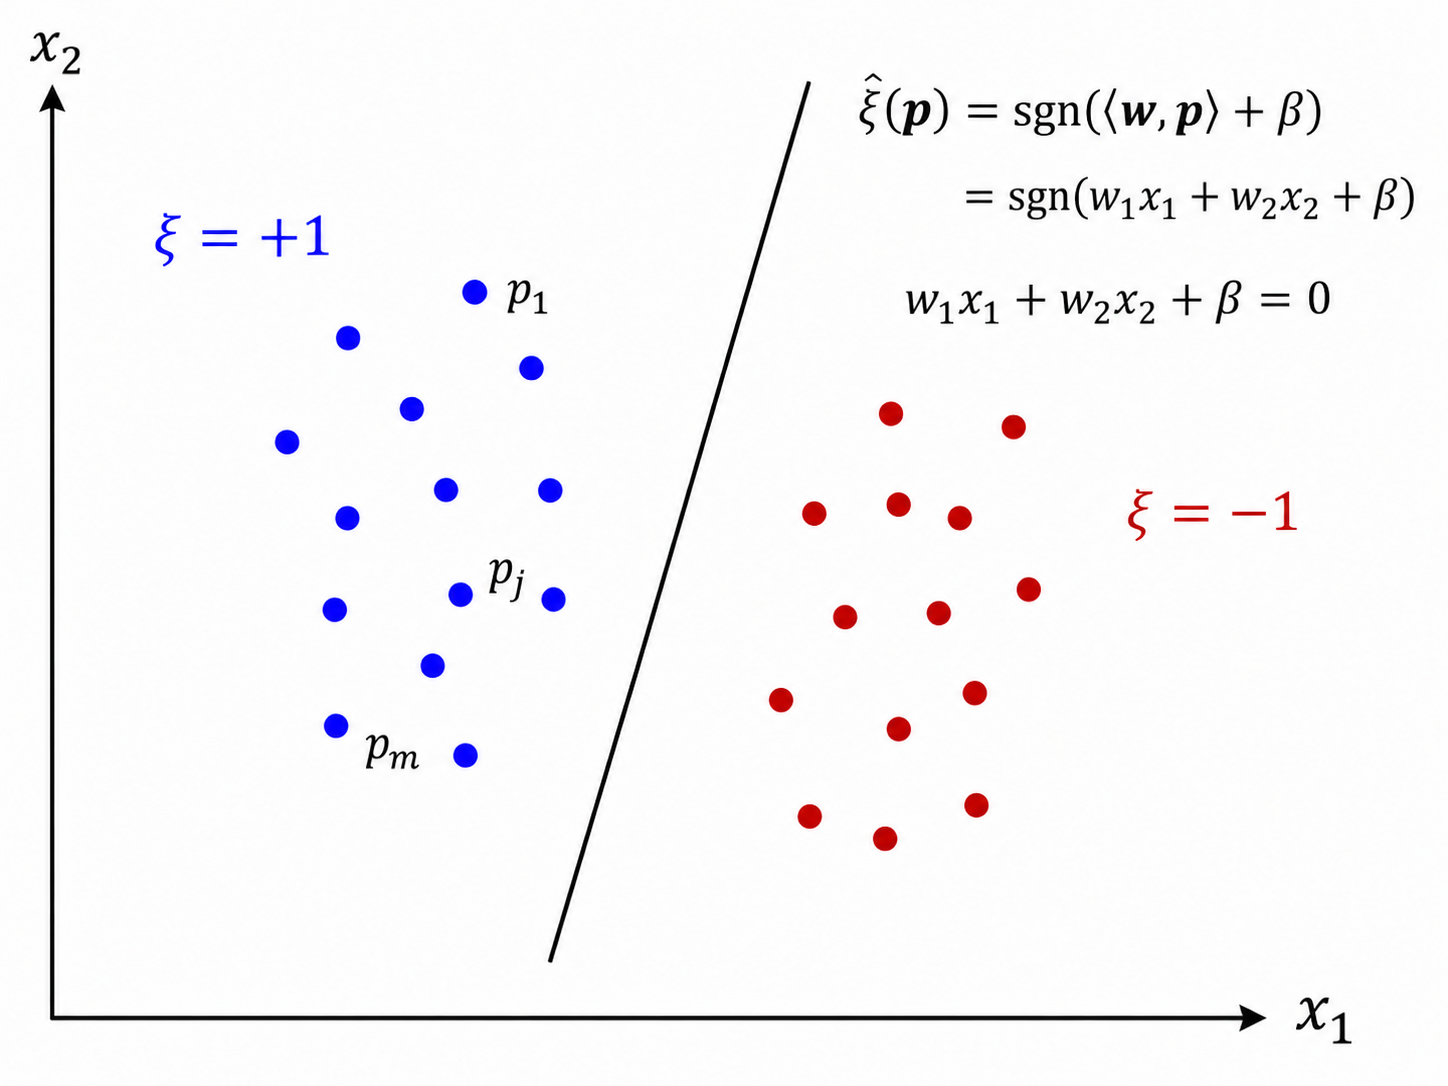
\includegraphics[
        width=1.06\linewidth,
        height=.74\paperheight,
        keepaspectratio
      ]{figures/2d.png}%
    }
  }

\SPBGContentSlide
  {Задача классификации в трёхмерном случае}
  {%
    \centering
    \makebox[\linewidth][c]{%
      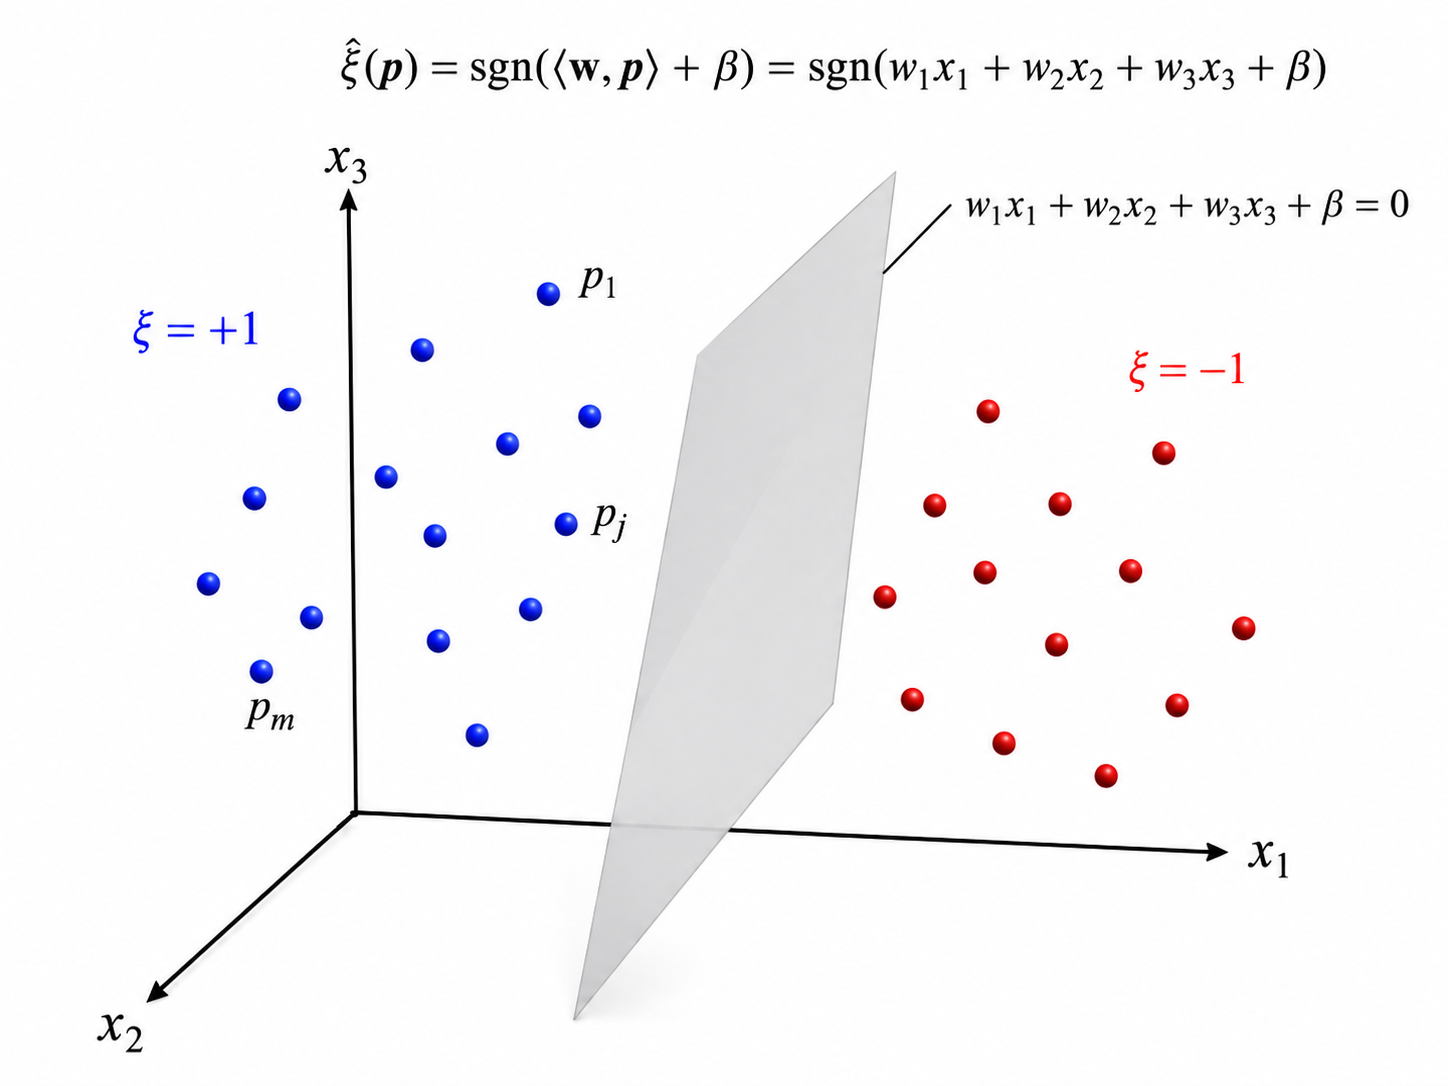
\includegraphics[
        width=1.06\linewidth,
        height=.74\paperheight,
        keepaspectratio
      ]{figures/3d.png}%
    }
  }

\SPBGSectionSlide
  {{Метод опорных векторов (support vector machine, SVM)}}
  {Строгое и мягкое линейное отделение}

\SPBGContentSlide
  {Строгое линейное отделение}
  {%
    \SmallBody
    Рассмотрим два конечных множества точек и метки классов:
    \[
      P_1=\{p_j\}_{j=1}^{s},
      \qquad
      P_2=\{p_j\}_{j=s+1}^{m},
      \qquad
      \xi_j=\begin{cases}
        +1,& j=1,\ldots,s,\\
        -1,& j=s+1,\ldots,m.
      \end{cases}
    \]

    Гиперплоскость задаётся уравнением
    \[
      \langle w,p\rangle+\beta=0,
      \qquad
      w\in\mathbb{R}^{n},\quad w\neq0.
    \]

    Множества \(P_1\) и \(P_2\) допускают строгое линейное отделение,
    если существуют \(w\neq0\) и \(\beta\), такие что
    \[
      \begin{aligned}
        \langle w,p_j\rangle+\beta&>0,
        &&j=1,\ldots,s,\\
        \langle w,p_j\rangle+\beta&<0,
        &&j=s+1,\ldots,m.
      \end{aligned}
    \]

  }

\SPBGContentSlide
  {Каноническая нормировка}
  {%
    \SmallBody
    Одна и та же гиперплоскость не имеет единственной записи:
    \[
      \langle w,p\rangle+\beta=0
      \quad\Longleftrightarrow\quad
      \langle cw,p\rangle+c\beta=0,\qquad c>0.
    \]

    Чтобы зафиксировать масштаб параметров, вводят нормированные условия:
    \[
      \langle w,p_j\rangle+\beta\geq1,\quad j=1,\ldots,s,
      \qquad
      \langle w,p_j\rangle+\beta\leq-1,\quad j=s+1,\ldots,m.
    \]

    Или, используя метки классов:
    \[
      \xi_j\bigl(\langle w,p_j\rangle+\beta\bigr)\geq1,
      \qquad j=1,\ldots,m.
    \]
  }
\SPBGSplitSlide
  {Границы разделяющей полосы}
  {.330}{.50}
  {%
    \ReportSvmMargin
  }
  {.785}{.33}
  {%
    \SplitBody
    В нормированной записи рассматриваются три параллельные гиперплоскости:
    \[
      \begin{aligned}
        L_1&:\ \langle w,p\rangle+\beta=1,\\
        L_0&:\ \langle w,p\rangle+\beta=0,\\
        L_2&:\ \langle w,p\rangle+\beta=-1.
      \end{aligned}
    \]

    \begin{itemize}
  \item \(L_0\) -- разделяющая гиперплоскость;
  \item \(L_1\) и \(L_2\) -- границы разделяющей полосы.
\end{itemize}

    Можно доказать, что расстояние между границами равно
    \[
      h=\rho(L_1,L_2)=\frac{2}{\|w\|}.
    \]
  }

\SPBGContentSlide
  {SVM строгого отделения}
  {%
    \FormulaBody

    В канонической нормировке задача SVM записывается как

    \CenteredDisplayFormula{
      \min\limits_{w,\beta}\ \frac12\|w\|^2, \\[0.55em]
      \xi_j\bigl(\langle w,p_j\rangle+\beta\bigr)\geq 1,
      \quad j=1,\ldots,m.
    }

    \vspace{.35cm}

    \begin{itemize}
      \item \(w\in\mathbb{R}^n\), \(\beta\in\mathbb{R}\) -- параметры гиперплоскости;
      \item \(\langle w,p\rangle+\beta=0\) -- разделяющая гиперплоскость;
      \item минимизация \(\frac12\|w\|^2\) эквивалентна максимизации ширины полосы.
    \end{itemize}
  }

\SPBGContentSlide
  {Двойственная задача SVM}
  {%
    \FormulaBody
    Для строгого отделения лагранжиан имеет вид
    \[
      \mathcal{L}(w,\beta,\alpha)=
      \frac12\|w\|^2-
      \sum_{j=1}^{m}\alpha_j
      \bigl(\xi_j(\langle w,p_j\rangle+\beta)-1\bigr).
    \]

    Условия стационарности дают
    \[
      w=\sum_{j=1}^{m}\alpha_j\xi_jp_j,
      \qquad
      \sum_{j=1}^{m}\alpha_j\xi_j=0.
    \]

    Поэтому задача переходит к поиску коэффициентов \(\alpha_j\):
    \[
      \frac12\langle A_0^TA_0\alpha,\alpha\rangle-\sum_{j=1}^{m}\alpha_j
      \to\min,\quad
      \sum_{j=1}^{m}\xi_j\alpha_j=0,\quad \alpha_j\ge0.
    \]
  }


\SPBGSplitSlide
  {Опорные векторы}
  {.335}{.52}
  {%
    \ReportSvmSupportVectors
  }
  {.790}{.30}
  {%
    \SplitBody
    Обведённые точки лежат на границах разделяющей полосы.

    \vspace{.35cm}
    Для них выполняется
    \[
      \alpha_j>0.
    \]

    \vspace{.25cm}
    Именно они входят в представление нормали \(w^*\).
  }

\SPBGSplitSlide
  {Мягкое отделение}
  {.335}{.52}
  {%
    \ReportSoftMargin
  }
  {.785}{.31}
  {%
    \SplitBody
    Вводятся переменные нарушений:
    \[
      \begin{aligned}
      \xi_j(\langle w,p_j\rangle+\beta)&\geq 1-\eta_j,\\
      \eta_j&\geq0.
      \end{aligned}
    \]

    Прямая задача:
    \[
      \begin{aligned}
      \min_{w,\beta,\eta}\quad&
        \frac12\|w\|^2+C\sum_{j=1}^{m}\eta_j
      \end{aligned}
    \]

    \SplitBody
    Параметр \(C\) задаёт баланс между шириной полосы и штрафом за нарушения.
  }

\SPBGContentSlide
  {Двойственная задача мягкого отделения}
  {%
    \FormulaBody
    Переменные нарушений добавляют верхнюю границу для двойственных
    коэффициентов:
    \[
      0\leq \alpha_j\leq C,\qquad j=1,\ldots,m.
    \]

    Двойственная постановка сохраняет тот же квадратичный функционал:
    \[
      \frac12\langle A_0^TA_0\alpha,\alpha\rangle-
      \sum_{j=1}^{m}\alpha_j
      \to\min.
    \]

    Но допустимое множество становится ограниченным:
    \[
      \sum_{j=1}^{m}\xi_j\alpha_j=0,
      \qquad
      0\leq\alpha_j\leq C.
    \]

    \Body
    Это ограничивает влияние выбросов и объектов, попавших внутрь полосы.
  }


\SPBGSectionSlide
  {Обобщенный метод MDM}
  {Ближайшие точки выпуклых оболочек и восстановление разделителя}

\SPBGContentSlide
  {MDM: ближайшие точки выпуклых оболочек}
  {%
    \ReportMdmHulls
  }

\SPBGContentSlide
  {MDM: основная задача}
  {%
    \FormulaBody
    Каждому классу сопоставляются выпуклые оболочки
    \[
      C_1=\operatorname{conv}\{p_1,\ldots,p_s\},
      \qquad
      C_2=\operatorname{conv}\{p_{s+1},\ldots,p_m\}.
    \]

    MDM ищет ближайшие точки этих оболочек:
    \[
      \frac12\|w_1-w_2\|^2\to\min,
      \qquad
      w_1\in C_1,\quad w_2\in C_2.
    \]

    Через единый план \(u\) это записывается как
    \[
      Q(u)=\frac12\|Au\|^2\to\min,\qquad u\in U.
    \]

    \Body
    Вектор \(Au\) является текущим направлением между двумя оболочками.
  }


\SPBGContentSlide
  {Оценка оптимальности в MDM}
  {%
    \FormulaBody
    На итерации \(k\) текущий вектор \(w_k=Au_k\) задает направление,
    по которому выбираются две точки внутри одного класса:
    \[
      p'_k\in M_i^+(u_k),
      \qquad
      p''_k\in M_i^-.
    \]

    Величина
    \[
      \Delta_k=
      \langle w_k,p'_k-p''_k\rangle
    \]
    показывает, насколько можно уменьшить функционал переносом веса.

    \Body
    Если подходящего переноса уже нет, текущие точки оболочек удовлетворяют
    условию ближайшей пары и задают разделитель.
  }


\SPBGSplitSlide
  {Итерационный шаг MDM}
  {.335}{.52}
  {%
    \ReportMdmStep
  }
  {.790}{.30}
  {%
    \SplitBody
    Перенос веса:
    \[
      u_{k+1}
      =u_k+t_k u_{k,j'}(e_{j''}-e_{j'}).
    \]

    Длина шага:
    \[
      t_k=\min\left\{
        \frac{\Delta_k}{
          u_{k,j'}\|p_{j'}-p_{j''}\|^2},
        1
      \right\}.
    \]
  }

\SPBGSplitSlide
  {Восстановление гиперплоскости в MDM}
  {.335}{.50}
  {%
    \ReportMdmBridge
  }
  {.790}{.31}
  {%
    \SplitBody
    После нахождения ближайших точек
    \[
      w_1^*\in C_1,\qquad w_2^*\in C_2
    \]
    нормаль разделителя равна
    \[
      v=w_1^*-w_2^*.
    \]

    Центр полосы:
    \[
      c^*=\frac{w_1^*+w_2^*}{2}.
    \]

    Гиперплоскость:
    \[
      \langle v,p-c^*\rangle=0.
    \]
  }

\SPBGSectionSlide
  {MDM с мягким разделением}
  {Ограниченные веса и восстановление гиперплоскости}

\SPBGContentSlide
  {MDM с мягким разделением}
  {%
    \FormulaBody
    Мягкая двойственная постановка задаёт допустимое множество
    \[
      U=\left\{
        u\in\mathbb{R}^m\mid
        \sum_{j=1}^{m}\xi_j u_j=0,\;
        0\leq u_j\leq C
      \right\}.
    \]

    Целевая функция:
    \[
      D(u)=
      \frac12\langle A^TAu,u\rangle-\sum_{j=1}^{m}u_j
      \rightarrow \min,\qquad u\in U.
    \]

    Верхняя граница $u_j\leq C$ ограничивает влияние отдельного объекта.
  }

\SPBGContentSlide
  {Переход к мягкому MDM}
  {%
    \FormulaBody
    При пересечении классов ближайшие точки обычных оболочек уже не задают
    корректный разделитель. Поэтому используются ограниченные веса:
    \[
      U_C=\left\{
        u\in\mathbb{R}^m\mid
        \sum_{j=1}^{m}\xi_j u_j=0,\;
        0\le u_j\le C
      \right\}.
    \]

    Задача принимает вид
    \[
      D(u)=
      \frac12\langle A^TAu,u\rangle-
      \sum_{j=1}^{m}u_j
      \to\min,\qquad u\in U_C.
    \]

    \Body
    Верхняя граница \(C\) не дает одному объекту полностью определить
    положение разделяющей гиперплоскости.
  }


\SPBGContentSlide
  {Итерационный шаг мягкого MDM}
  {%
    \FormulaBody
    Шаг снова переносит вес между двумя координатами, но теперь учитывает
    нижнюю и верхнюю границы:
    \[
      0\leq u_j\leq C.
    \]

    Направление выбирается по производным целевой функции:
    \[
      q_j=\langle v,\xi_jp_j\rangle-1,
      \qquad
      v=Au.
    \]

    Для рабочей пары берется допустимое изменение, сохраняющее баланс
    \[
      \sum_{j=1}^{m}\xi_j u_j=0.
    \]

    \Body
    Поэтому мягкий вариант сохраняет идею MDM-переноса веса, но работает
    уже не с двумя непересекающимися оболочками, а с ограниченным
    допустимым множеством коэффициентов.
  }


\SPBGContentSlide
  {Гиперплоскость в мягкой постановке}
  {%
    \FormulaBody
    Нормаль после решения мягкой задачи восстанавливается по плану:
    \[
      w^*=Au^*=\sum_{j=1}^{m}u_j^*\xi_jp_j.
    \]

    Если найден объект с внутренним коэффициентом \(0<u_j^*<C\), то
    \[
      \beta^*=\xi_j-\langle w^*,p_j\rangle.
    \]

    Когда таких объектов нет, параметр \(\beta\) можно определить из
    одномерной вспомогательной задачи
    \[
      f(\beta)=
      \sum_{j=1}^{m}
      \bigl[1-\xi_j(\langle w^*,p_j\rangle+\beta)\bigr]_+
      \to\min.
    \]

    \Body
    Это завершает переход от найденных коэффициентов к классификатору.
  }


\SPBGSectionSlide
  {Модификации шага MDM}
  {Групповой, треугольный, циклический и комбинированный варианты}

\SPBGSplitSlide
  {Перенос веса в группу минимумов}
  {.315}{.52}
  {%
    \ReportGroupStep
  }
  {.790}{.34}
  {%
    \SplitBody
    В базовом MDM вес переносится к одной точке с минимальной проекцией.

    \vspace{.22cm}
    В модификации строится множество
    \[
      I_{\min}=\{j:\langle p_j,w_k\rangle
      =\min_i\langle p_i,w_k\rangle\}.
    \]

    Вместо одной точки используется центр группы
    \[
      \bar p_{\min}
      =\frac1{|I_{\min}|}\sum_{j\in I_{\min}}p_j.
    \]

    Кандидат шага строится в направлении
    \[
      d=\bar p_{\min}-p',
    \]
    а длина шага выбирается так, чтобы сохранить допустимость весов и
    уменьшить \(Q(u)\).
  }

\SPBGSplitSlide
  {Геометрический треугольный шаг}
  {.325}{.46}
  {%
    \ReportTriangleStep
  }
  {.785}{.34}
  {%
    \SplitBody
    Вместо движения по одному MDM-отрезку строятся несколько допустимых
    локальных направлений.

    \vspace{.18cm}
    Пусть \(r_k\) и \(q_k\) -- точки, полученные альтернативными переносами
    веса. Тогда рассматривается
    \[
      T_k=\operatorname{conv}\{w_k,r_k,q_k\}.
    \]

    Следующая точка выбирается как проекция нуля:
    \[
      \widetilde w_k
      =\arg\min_{w\in T_k}\|w\|^2.
    \]

    Если соответствующие веса допустимы, этот кандидат участвует в выборе
    шага.
  }

\SPBGSplitSlide
  {Ускорение по повторяющимся циклам}
  {.340}{.58}
  {%
    \ReportCycleAcceleration
  }
  {.805}{.30}
  {%
    \SplitBody
    Если последние направления начинают повторяться,
    \[
      s_k\approx s_{k-2},\qquad
      s_{k+1}\approx s_{k-1},
    \]
    строится суммарное смещение
    \[
      v_k=s_{k-2}+s_{k-1}.
    \]

    Ускоренный кандидат задаётся как
    \[
      \widetilde w_k=w_k+\rho_k v_k,
    \]
    где \(\rho_k\) выбирается из условия допустимости и уменьшения
    \(Q(u)\).

    Если такого уменьшения нет, используется обычный MDM-шаг.
  }

\SPBGContentSlide
  {Комбинированный выбор шага}
  {%
    \SmallBody
    Комбинированный вариант работает в той же допустимой области весов:
    \[
      u\in\Delta,\qquad
      0\le u_j\le C \quad \text{для мягкой постановки}.
    \]

    На каждой итерации строится набор допустимых кандидатов
    \(\mathcal U_k\):

    \vspace{.12cm}
    \begin{itemize}
      \item базовый перенос веса;
      \item групповой перенос;
      \item геометрический треугольный шаг;
      \item ускоренный шаг по циклу, если он доступен.
    \end{itemize}

    \vspace{.12cm}
    Выбор задаётся правилом
    \[
      u_{k+1}=\arg\min_{u\in\mathcal U_k}Q(u).
    \]

    Если дополнительные кандидаты не улучшают значение функционала,
    алгоритм возвращается к базовому MDM-шагу.
  }

\SPBGSectionSlide
  {SMO-алгоритм}
  {Парная оптимизация двойственной задачи SVM}


\SPBGContentSlide
  {SMO: парное изменение коэффициентов}
  {%
    \FormulaBody
    В двойственной задаче SVM действует ограничение баланса
    \[
      \sum_{j=1}^{m}\alpha_j\xi_j=0.
    \]

    Поэтому нетривиальный шаг должен менять минимум две координаты:
    \[
      \alpha_{i'}\leftarrow \alpha_{i'}+\xi_{i'}\lambda,
      \qquad
      \alpha_{i''}\leftarrow \alpha_{i''}-\xi_{i''}\lambda.
    \]

    Вектор нормали обновляется рекуррентно:
    \[
      v_{k+1}=v_k+\lambda(p_{i'}-p_{i''}).
    \]
  }

\SPBGContentSlide
  {SMO: допустимые планы}
  {%
    \FormulaBody
    SMO решает двойственную задачу SVM:
    \[
      D(\alpha)=
      \frac12\langle A_0^TA_0\alpha,\alpha\rangle-
      \sum_{j=1}^{m}\alpha_j
      \to\min.
    \]

    Допустимые планы должны сохранять баланс классов:
    \[
      \sum_{j=1}^{m}\xi_j\alpha_j=0.
    \]

    В мягкой постановке добавляются ограничения
    \[
      0\leq\alpha_j\leq C.
    \]

    \Body
    Поэтому одиночное изменение коэффициента обычно невозможно:
    нужен парный шаг.
  }


\SPBGContentSlide
  {Парная подзадача SMO}
  {%
    \FormulaBody
    На шаге выбираются индексы \(i'\) и \(i''\), а остальные коэффициенты
    считаются фиксированными:
    \[
      \alpha_{i'}\leftarrow \alpha_{i'}+\xi_{i'}\lambda,
      \qquad
      \alpha_{i''}\leftarrow \alpha_{i''}-\xi_{i''}\lambda.
    \]

    Параметр \(\lambda\) находится из одномерной квадратичной задачи и
    затем усекается так, чтобы остались выполнены границы
    \[
      0\leq\alpha_{i'},\alpha_{i''}\leq C.
    \]

    \Body
    Именно поэтому SMO удобен вычислительно: большая задача разбивается
    на последовательность очень малых подзадач.
  }


\SPBGContentSlide
  {Оптимальность и связь SMO с MDM}
  {%
    \FormulaBody
    В реализации контролируется разрыв между допустимыми направлениями:
    \[
      \Delta(\alpha)=
      \max_{j\in I''(\alpha)}q_j-
      \min_{j\in I'(\alpha)}q_j.
    \]

    Остановка выполняется при
    \[
      \Delta(\alpha)\leq\varepsilon.
    \]

    Нормаль восстанавливается так же, как в двойственной SVM:
    \[
      w^*=\sum_{j=1}^{m}\alpha_j^*\xi_jp_j.
    \]

    \Body
    По структуре шага SMO близок к MDM: оба метода меняют пару весов,
    но делают это в разных допустимых множествах.
  }


\SPBGSectionSlide
  {Экспериментальное сравнение}
  {Главный блок презентации: протокол, таблицы, графики и выводы}

\SPBGContentSlide
  {Протокол экспериментов}
  {%
    \Body
    Сравнение проводилось в двух режимах.

    \vspace{.25cm}
    \begin{itemize}
      \item \Accent{Строгое отделение}: разделимые синтетические наборы S1--S4;
      метрики -- итерации, время, ширина полосы, активные точки.
      \item \Purple{Мягкое отделение}: неразделимые синтетические наборы N1--N4
      и реальные бинарные датасеты R1--R15;
      метрики -- Test F1, ROC-AUC, время.
    \end{itemize}

    \vspace{.25cm}
    Для неразделимых и реальных данных использовалось стратифицированное
    разбиение $70/30$. В мягкой постановке фиксировалось $C=1$.
  }

\SPBGContentSlide
  {Типы данных в эксперименте}
  {%
    \centering
    \begin{tikzpicture}[>=Latex, every node/.style={font=\fontsize{15}{18}\selectfont}]
      \node[draw=spbgeuTeal!70, fill=spbgeuTeal!10, rounded corners=4pt,
        text width=3.8cm, minimum height=2.35cm, align=center] (s) at (-4.35,1.15)
        {\bfseries S1--S4\\[3pt]разделимая\\синтетика};
      \node[draw=spbgeuPurple!70, fill=spbgeuPurple!10, rounded corners=4pt,
        text width=3.9cm, minimum height=2.35cm, align=center] (n) at (0,1.15)
        {\bfseries N1--N4\\[3pt]пересечения, выбросы,\\шум, XOR};
      \node[draw=spbgeuText!55, fill=gray!12, rounded corners=4pt,
        text width=3.9cm, minimum height=2.35cm, align=center] (r) at (4.35,1.15)
        {\bfseries R1--R15\\[3pt]реальные бинарные\\датасеты};

      \node[text=spbgeuTeal, text width=3.4cm, align=center] (sd) at (-4.35,-2.00)
        {геометрия\\строгого отделения};
      \node[text=spbgeuPurple, text width=3.6cm, align=center] (nd) at (0,-2.00)
        {качество при\\пересечении классов};
      \node[text=spbgeuText, text width=3.8cm, align=center] (rd) at (4.35,-2.00)
        {устойчивость\\на практике};

      \draw[->, thick, spbgeuTeal] (s.south) to[out=-85,in=105] (sd.north);
      \draw[->, thick, spbgeuPurple] (n.south) to[out=-90,in=90] (nd.north);
      \draw[->, thick, spbgeuText] (r.south) to[out=-95,in=75] (rd.north);
    \end{tikzpicture}
  }

\SPBGContentSlide
  {Методы и обозначения}
  {%
    \centering
    \SmallBody
    \renewcommand{\arraystretch}{1.08}
    \begin{tabularx}{.95\linewidth}{@{}l>{\raggedright\arraybackslash}X>{\raggedright\arraybackslash}X@{}}
      \toprule
      Код & Метод & Смысл шага \\
      \midrule
      H1 & Базовый MDM & перенос веса между двумя точками \\
      H2 & SMO & парное изменение двойственных коэффициентов \\
      H3 & MDM-G & перенос в группу минимумов \\
      H4 & MDM-A & ускорение по повторяющимся циклам \\
      H5 & Треугольный MDM & выбор ближайшей точки локального треугольника \\
      H6 & Комбинированный MDM & выбор лучшего из нескольких кандидатов \\
      \bottomrule
    \end{tabularx}
  }

\SPBGContentSlide
  {Методы и обозначения}
  {%
    \centering
    \SmallBody
    \renewcommand{\arraystretch}{1.15}
    \begin{tabularx}{.95\linewidth}{@{}>{\raggedright\arraybackslash}X>{\raggedright\arraybackslash}X>{\raggedright\arraybackslash}X@{}}
      \toprule
      Обозначения & Группа методов & Постановка \\
      \midrule
      MDM, MDM-G, MDM-A & мягкие MDM-варианты & ограничения $0\leq u_j\leq C$ \\
      SMO, SVC, LinearSVC & SVM-решатели & мягкая линейная постановка \\
      \bottomrule
    \end{tabularx}
  }

\SPBGContentSlide
  {Метрики качества}
  {%
    \FormulaBody
    Для мягкой постановки использовались две основные test-метрики:
    \[
      F_1=
      2\cdot
      \frac{\mathrm{Precision}\cdot\mathrm{Recall}}
      {\mathrm{Precision}+\mathrm{Recall}},
      \qquad
      \mathrm{ROC\text{-}AUC}
      =
      \int_0^1 TPR(FPR)\,dFPR.
    \]

    \vspace{.15cm}
    \Body
    F1 фиксирует качество итоговой бинарной классификации,
    а ROC-AUC оценивает способность метода правильно ранжировать объекты.
  }

\SPBGContentSlide
  {Строгое отделение: средние результаты}
  {%
    \centering
    \Body
    \renewcommand{\arraystretch}{1.18}
    \setlength{\tabcolsep}{10pt}
    \begin{tabular}{|l|r|r|r|}
      \hline
      Метод & Итерации & Время, с & Train acc. \\
      \hline
      Базовый MDM & 672.4 & 0.0584 & 1.000 \\
      \hline
      SMO & 256.7 & 0.0068 & 1.000 \\
      \hline
      MDM-G & 690.2 & 0.0792 & 1.000 \\
      \hline
      MDM-A & 565.7 & 0.0719 & 1.000 \\
      \hline
      Треугольный MDM & 307.1 & 0.0533 & 1.000 \\
      \hline
      Комбинированный MDM & 217.1 & 0.1259 & 1.000 \\
      \hline
    \end{tabular}
  }

\ChartFrame{Строгое отделение: число итераций}{%
  \begin{tikzpicture}
    \begin{axis}[
      width=.92\textwidth,
      height=.58\paperheight,
      grid=major,
      major grid style={gray!20},
      ybar,
      ymin=0,
      ylabel={Среднее число итераций},
      symbolic x coords={H1,H2,H3,H4,H5,H6},
      xtick=data,
      bar width=14pt,
      scaled y ticks=false
    ]
      \addplot[fill=spbgeuTeal!55, draw=spbgeuTeal] coordinates
        {(H1,672.4) (H2,256.7) (H3,690.2) (H4,565.7) (H5,307.1) (H6,217.1)};
    \end{axis}
  \end{tikzpicture}
}

\ChartFrame{Строгое отделение: время обучения}{%
  \begin{tikzpicture}
    \begin{axis}[
      width=.92\textwidth,
      height=.58\paperheight,
      grid=major,
      major grid style={gray!20},
      ybar,
      ymin=0,
      ylabel={Среднее время, с},
      symbolic x coords={H1,H2,H3,H4,H5,H6},
      xtick=data,
      bar width=14pt,
      scaled y ticks=false
    ]
      \addplot[fill=spbgeuPurple!50, draw=spbgeuPurple] coordinates
        {(H1,0.0584) (H2,0.0068) (H3,0.0792) (H4,0.0719) (H5,0.0533) (H6,0.1259)};
    \end{axis}
  \end{tikzpicture}
}

\ChartFrame{Строгое отделение: зависимость от набора}{%
  \begin{tikzpicture}
    \begin{axis}[
      width=.92\textwidth,
      height=.58\paperheight,
      grid=major,
      major grid style={gray!20},
      ybar,
      ymin=0,
      ylabel={Итерации},
      symbolic x coords={S1,S2,S3,S4},
      xtick=data,
      bar width=5pt,
      legend style={at={(0.5,-0.18)}, anchor=north, legend columns=6, font=\small, \SPBGLegendPlaque}
    ]
      \addplot[fill=blue!45] coordinates {(S1,564.9) (S2,955.1) (S3,375.6) (S4,794.0)};
      \addplot[fill=black!45] coordinates {(S1,21.1) (S2,674.7) (S3,15.8) (S4,315.1)};
      \addplot[fill=red!45] coordinates {(S1,564.9) (S2,1025.1) (S3,375.6) (S4,795.2)};
      \addplot[fill=green!45] coordinates {(S1,564.9) (S2,592.9) (S3,375.6) (S4,729.3)};
      \addplot[fill=orange!65] coordinates {(S1,3.2) (S2,531.9) (S3,3.2) (S4,690.1)};
      \addplot[fill=spbgeuPurple!55] coordinates {(S1,3.1) (S2,230.0) (S3,3.0) (S4,632.2)};
      \legend{H1,H2,H3,H4,H5,H6}
    \end{axis}
  \end{tikzpicture}
}

\ChartFrame{Относительное ускорение по итерациям}{%
  \begin{tikzpicture}
    \begin{axis}[
      width=.92\textwidth,
      height=.58\paperheight,
      grid=major,
      major grid style={gray!20},
      ybar,
      ymode=log,
      ymin=.8,
      ylabel={$I_{H1}/I_M$},
      symbolic x coords={S1,S2,S3,S4},
      xtick=data,
      bar width=5pt,
      legend style={at={(0.5,-0.18)}, anchor=north, legend columns=6, font=\small, \SPBGLegendPlaque}
    ]
      \addplot[fill=blue!45] coordinates {(S1,1.0) (S2,1.0) (S3,1.0) (S4,1.0)};
      \addplot[fill=black!45] coordinates {(S1,26.8) (S2,1.4) (S3,23.8) (S4,2.5)};
      \addplot[fill=red!45] coordinates {(S1,1.0) (S2,.93) (S3,1.0) (S4,1.0)};
      \addplot[fill=green!45] coordinates {(S1,1.0) (S2,1.6) (S3,1.0) (S4,1.1)};
      \addplot[fill=orange!65] coordinates {(S1,175.3) (S2,1.8) (S3,116.6) (S4,1.2)};
      \addplot[fill=spbgeuPurple!55] coordinates {(S1,181.6) (S2,4.2) (S3,125.2) (S4,1.3)};
      \legend{H1,H2,H3,H4,H5,H6}
    \end{axis}
  \end{tikzpicture}
}

\ChartFrame{Влияние размера выборки}{%
  \begin{tikzpicture}
    \begin{axis}[
      width=.92\textwidth,
      height=.58\paperheight,
      grid=major,
      major grid style={gray!20},
      xlabel={Объектов на класс},
      ylabel={Итерации},
      legend style={at={(0.5,-0.18)}, anchor=north, legend columns=6, font=\small, \SPBGLegendPlaque}
    ]
      \addplot+[mark=*, thick, blue] coordinates {(100,271.6) (250,721.3) (500,1024.3)};
      \addplot+[mark=star, thick, black] coordinates {(100,182.8) (250,333.1) (500,254.2)};
      \addplot+[mark=square*, thick, red] coordinates {(100,266.3) (250,777.1) (500,1027.3)};
      \addplot+[mark=triangle*, thick, green!60!black] coordinates {(100,217.8) (250,522.2) (500,957.1)};
      \addplot+[mark=diamond*, thick, orange!80!black] coordinates {(100,128.8) (250,374.2) (500,418.3)};
      \addplot+[mark=o, thick, spbgeuPurple] coordinates {(100,111.9) (250,207.4) (500,331.9)};
      \legend{H1,H2,H3,H4,H5,H6}
    \end{axis}
  \end{tikzpicture}
}

\ChartFrame{Влияние размерности: итерации}{%
  \begin{tikzpicture}
    \begin{axis}[
      width=.92\textwidth,
      height=.58\paperheight,
      grid=major,
      major grid style={gray!20},
      xlabel={Размерность $d$},
      ylabel={Итерации},
      legend style={at={(0.5,-0.18)}, anchor=north, legend columns=6, font=\small, \SPBGLegendPlaque}
    ]
      \addplot+[mark=*, thick, blue] coordinates {(2,239) (5,537.3) (10,619.7) (20,1296.7) (50,1883.7) (100,3347.7)};
      \addplot+[mark=star, thick, black] coordinates {(2,61) (5,694.3) (10,681) (20,1296.7) (50,1984) (100,2849.7)};
      \addplot+[mark=square*, thick, red] coordinates {(2,238.7) (5,522.3) (10,630.7) (20,1305.3) (50,1889.7) (100,3338.3)};
      \addplot+[mark=triangle*, thick, green!60!black] coordinates {(2,239) (5,384.7) (10,506) (20,937.7) (50,1369) (100,2281.7)};
      \addplot+[mark=diamond*, thick, orange!80!black] coordinates {(2,48.7) (5,355.7) (10,554.7) (20,1308.7) (50,2248) (100,3683.3)};
      \addplot+[mark=o, thick, spbgeuPurple] coordinates {(2,46.7) (5,258) (10,431) (20,835.3) (50,1415) (100,2359.7)};
      \legend{H1,H2,H3,H4,H5,H6}
    \end{axis}
  \end{tikzpicture}
}

\ChartFrame{Влияние размерности: время}{%
  \begin{tikzpicture}
    \begin{axis}[
      width=.92\textwidth,
      height=.58\paperheight,
      grid=major,
      major grid style={gray!20},
      xlabel={Размерность $d$},
      ylabel={Время, с},
      legend style={at={(0.5,-0.18)}, anchor=north, legend columns=6, font=\small, \SPBGLegendPlaque}
    ]
      \addplot+[mark=*, thick, blue] coordinates {(2,0.0156) (5,0.0320) (10,0.0385) (20,0.0845) (50,0.1482) (100,0.3367)};
      \addplot+[mark=star, thick, black] coordinates {(2,0.0015) (5,0.0161) (10,0.0160) (20,0.0311) (50,0.0496) (100,0.0718)};
      \addplot+[mark=square*, thick, red] coordinates {(2,0.0209) (5,0.0417) (10,0.0514) (20,0.1117) (50,0.1956) (100,0.4356)};
      \addplot+[mark=triangle*, thick, green!60!black] coordinates {(2,0.0196) (5,0.0349) (10,0.0480) (20,0.0942) (50,0.1602) (100,0.3217)};
      \addplot+[mark=diamond*, thick, orange!80!black] coordinates {(2,0.0058) (5,0.0422) (10,0.0695) (20,0.1716) (50,0.3483) (100,0.6979)};
      \addplot+[mark=o, thick, spbgeuPurple] coordinates {(2,0.0161) (5,0.0930) (10,0.1640) (20,0.3405) (50,0.6749) (100,1.3840)};
      \legend{H1,H2,H3,H4,H5,H6}
    \end{axis}
  \end{tikzpicture}
}

\SPBGContentSlide
  {Контроль геометрического решения}
  {%
    \centering
    \Body
    \renewcommand{\arraystretch}{1.2}
    \setlength{\tabcolsep}{9pt}
    \begin{tabular}{|r|r|r|r|r|}
      \hline
      $d$ & Ширина MDM & Ширина SVC & Активные MDM & Опорные SVC \\
      \hline
      2 & 3.095 & 3.094 & 3.0 & 3.0 \\
      \hline
      5 & 3.151 & 3.151 & 5.7 & 5.7 \\
      \hline
      10 & 3.201 & 3.201 & 9.7 & 9.7 \\
      \hline
      20 & 3.330 & 3.330 & 17.0 & 17.3 \\
      \hline
      50 & 3.478 & 3.478 & 33.7 & 34.0 \\
      \hline
      100 & 3.637 & 3.637 & 66.7 & 66.7 \\
      \hline
    \end{tabular}
  }

\SPBGContentSlide
  {Мягкое отделение: синтетика}
  {%
    \centering
    \Body
    \renewcommand{\arraystretch}{1.16}
    \setlength{\tabcolsep}{8pt}
    \begin{tabular}{|l|r|r|r|r|}
      \hline
      Метод & Test F1 & ROC-AUC & Время, с & Итерации \\
      \hline
      Мягкий MDM & 0.647 & 0.749 & 0.2997 & 310.9 \\
      \hline
      Мягкий MDM-G & 0.647 & 0.749 & 0.6601 & 313.4 \\
      \hline
      Мягкий MDM-A & 0.615 & 0.685 & 1.2505 & 255.1 \\
      \hline
      Мягкий SMO & 0.808 & 0.777 & 0.0362 & 1283.4 \\
      \hline
      SVC & 0.808 & 0.777 & 0.0018 & -- \\
      \hline
      LinearSVC & 0.751 & 0.778 & 0.0004 & 3.5 \\
      \hline
    \end{tabular}
  }

\ChartFrame{Неразделимые данные: качество и время}{%
  \begin{tikzpicture}
    \begin{axis}[
      width=.92\textwidth,
      height=.58\paperheight,
      grid=major,
      major grid style={gray!20},
      xmode=log,
      xmin=0.0002,
      xmax=2.0,
      ymin=.55,
      ymax=.84,
      xlabel={Время, с},
      ylabel={Test F1}
    ]
      \addplot+[only marks, mark=*, mark size=3.8pt, blue] coordinates {(0.2997,0.647)};
      \node[font=\scriptsize, blue, anchor=south east] at (axis cs:0.2997,0.647) {MDM};
      \addplot+[only marks, mark=diamond*, mark size=3.8pt, spbgeuTeal] coordinates {(0.6601,0.647)};
      \node[font=\scriptsize, spbgeuTeal, anchor=south west] at (axis cs:0.6601,0.647) {MDM-G};
      \addplot+[only marks, mark=o, mark size=3.8pt, spbgeuPurple] coordinates {(1.2505,0.615)};
      \node[font=\scriptsize, spbgeuPurple, anchor=north west] at (axis cs:1.2505,0.615) {MDM-A};
      \addplot+[only marks, mark=star, mark size=4pt, black] coordinates {(0.0362,0.808)};
      \node[font=\scriptsize, anchor=south west] at (axis cs:0.0362,0.808) {SMO};
      \addplot+[only marks, mark=square*, mark size=3.8pt, red] coordinates {(0.0018,0.808)};
      \node[font=\scriptsize, red, anchor=south west] at (axis cs:0.0018,0.808) {SVC};
      \addplot+[only marks, mark=triangle*, mark size=3.8pt, green!60!black] coordinates {(0.0004,0.751)};
      \node[font=\scriptsize, green!45!black, anchor=south west] at (axis cs:0.0004,0.751) {LinearSVC};
    \end{axis}
  \end{tikzpicture}
}

\ChartFrame{Неразделимые данные: F1 по наборам}{%
  \begin{tikzpicture}
    \begin{axis}[
      width=.92\textwidth,
      height=.58\paperheight,
      grid=major,
      major grid style={gray!20},
      ybar,
      ymin=0,
      ymax=1,
      ylabel={Test F1},
      symbolic x coords={N1,N2,N3,N4},
      xtick=data,
      bar width=5pt,
      legend style={at={(0.5,-0.18)}, anchor=north, legend columns=3, font=\small, \SPBGLegendPlaque}
    ]
      \addplot[fill=blue!45] coordinates {(N1,0.754) (N2,0.864) (N3,0.780) (N4,0.189)};
      \addplot[fill=spbgeuPurple!45] coordinates {(N1,0.646) (N2,0.809) (N3,0.774) (N4,0.232)};
      \addplot[fill=black!45] coordinates {(N1,0.751) (N2,0.894) (N3,0.874) (N4,0.714)};
      \addplot[fill=red!45] coordinates {(N1,0.751) (N2,0.894) (N3,0.874) (N4,0.714)};
      \addplot[fill=green!45] coordinates {(N1,0.750) (N2,0.894) (N3,0.872) (N4,0.490)};
      \legend{MDM,MDM-A,SMO,SVC,LinearSVC}
    \end{axis}
  \end{tikzpicture}
}

\ChartFrame{Неразделимые данные: F1 и размер выборки}{%
  \begin{tikzpicture}
    \begin{axis}[
      width=.92\textwidth,
      height=.58\paperheight,
      grid=major,
      major grid style={gray!20},
      xlabel={Объектов на класс},
      ylabel={Test F1},
      ymin=.54,
      ymax=.84,
      legend style={at={(0.5,-0.18)}, anchor=north, legend columns=3, font=\small, \SPBGLegendPlaque}
    ]
      \addplot+[mark=*, thick, blue] coordinates {(100,0.698) (250,0.629) (500,0.614)};
      \addplot+[mark=diamond*, thick, spbgeuTeal] coordinates {(100,0.698) (250,0.629) (500,0.614)};
      \addplot+[mark=o, thick, spbgeuPurple] coordinates {(100,0.698) (250,0.576) (500,0.572)};
      \addplot+[mark=star, thick, black] coordinates {(100,0.793) (250,0.820) (500,0.811)};
      \addplot+[mark=square*, thick, red] coordinates {(100,0.793) (250,0.820) (500,0.811)};
      \addplot+[mark=triangle*, thick, green!60!black] coordinates {(100,0.744) (250,0.760) (500,0.750)};
      \legend{MDM,MDM-G,MDM-A,SMO,SVC,LinearSVC}
    \end{axis}
  \end{tikzpicture}
}

\SPBGContentSlide
  {Реальные бинарные данные}
  {%
    \centering
    \SmallBody
    \renewcommand{\arraystretch}{1.16}
    \begin{tabular}{@{}lrrrr@{}}
      \toprule
      Метод & Test F1 & ROC-AUC & Время, с & Итерации \\
      \midrule
      Мягкий MDM & 0.823 & 0.919 & 1.5123 & 554.4 \\
      Мягкий MDM-G & 0.823 & 0.920 & 3.1236 & 558.1 \\
      Мягкий MDM-A & 0.822 & 0.921 & 6.3971 & 499.3 \\
      Мягкий SMO & 0.815 & 0.909 & 0.2357 & 3421.5 \\
      SVC & 0.844 & 0.924 & 0.1988 & -- \\
      LinearSVC & 0.846 & 0.925 & 0.0027 & 12.6 \\
      \bottomrule
    \end{tabular}
  }

\ChartFrame{Реальные данные: качество и время}{%
  \begin{tikzpicture}
    \begin{axis}[
      width=.92\textwidth,
      height=.58\paperheight,
      grid=major,
      major grid style={gray!20},
      xmode=log,
      xmin=0.001,
      xmax=9,
      ymin=.78,
      ymax=.86,
      xlabel={Время, с},
      ylabel={Test F1}
    ]
      \addplot+[only marks, mark=*, mark size=3.8pt, blue] coordinates {(1.5123,0.823)};
      \node[font=\scriptsize, blue, anchor=south east] at (axis cs:1.5123,0.823) {MDM};
      \addplot+[only marks, mark=diamond*, mark size=3.8pt, spbgeuTeal] coordinates {(3.1236,0.823)};
      \node[font=\scriptsize, spbgeuTeal, anchor=south] at (axis cs:3.1236,0.823) {MDM-G};
      \addplot+[only marks, mark=o, mark size=3.8pt, spbgeuPurple] coordinates {(6.3971,0.822)};
      \node[font=\scriptsize, spbgeuPurple, anchor=south west] at (axis cs:6.3971,0.822) {MDM-A};
      \addplot+[only marks, mark=star, mark size=4pt, black] coordinates {(0.2357,0.815)};
      \node[font=\scriptsize, anchor=north west] at (axis cs:0.2357,0.815) {SMO};
      \addplot+[only marks, mark=square*, mark size=3.8pt, red] coordinates {(0.1988,0.844)};
      \node[font=\scriptsize, red, anchor=south west] at (axis cs:0.1988,0.844) {SVC};
      \addplot+[only marks, mark=triangle*, mark size=3.8pt, green!60!black] coordinates {(0.0027,0.846)};
      \node[font=\scriptsize, green!45!black, anchor=south west] at (axis cs:0.0027,0.846) {LinearSVC};
    \end{axis}
  \end{tikzpicture}
}

\ChartFrame{Реальные данные: F1 при разной доле объектов}{%
  \begin{tikzpicture}
    \begin{axis}[
      width=.92\textwidth,
      height=.58\paperheight,
      grid=major,
      major grid style={gray!20},
      xlabel={Доля данных, \%},
      ylabel={Test F1},
      ymin=.78,
      ymax=.87,
      legend style={at={(0.5,-0.18)}, anchor=north, legend columns=3, font=\small, \SPBGLegendPlaque}
    ]
      \addplot+[mark=*, thick, blue] coordinates {(20,0.817) (50,0.829)};
      \addplot+[mark=diamond*, thick, spbgeuTeal] coordinates {(20,0.817) (50,0.829)};
      \addplot+[mark=o, thick, spbgeuPurple] coordinates {(20,0.816) (50,0.828)};
      \addplot+[mark=star, thick, black] coordinates {(20,0.837) (50,0.794)};
      \addplot+[mark=square*, thick, red] coordinates {(20,0.860) (50,0.828)};
      \addplot+[mark=triangle*, thick, green!60!black] coordinates {(20,0.853) (50,0.839)};
      \legend{MDM,MDM-G,MDM-A,SMO,SVC,LinearSVC}
    \end{axis}
  \end{tikzpicture}
}

\ChartFrame{Реальные данные: время при разной доле объектов}{%
  \begin{tikzpicture}
    \begin{axis}[
      width=.92\textwidth,
      height=.58\paperheight,
      grid=major,
      major grid style={gray!20},
      ymode=log,
      xlabel={Доля данных, \%},
      ylabel={Время, с},
      legend style={at={(0.5,-0.18)}, anchor=north, legend columns=3, font=\small, \SPBGLegendPlaque}
    ]
      \addplot+[mark=*, thick, blue] coordinates {(20,0.6551) (50,2.3694)};
      \addplot+[mark=diamond*, thick, spbgeuTeal] coordinates {(20,1.3960) (50,4.8512)};
      \addplot+[mark=o, thick, spbgeuPurple] coordinates {(20,2.7937) (50,10.0004)};
      \addplot+[mark=star, thick, black] coordinates {(20,0.1786) (50,0.2928)};
      \addplot+[mark=square*, thick, red] coordinates {(20,0.0536) (50,0.3441)};
      \addplot+[mark=triangle*, thick, green!60!black] coordinates {(20,0.0018) (50,0.0036)};
      \legend{MDM,MDM-G,MDM-A,SMO,SVC,LinearSVC}
    \end{axis}
  \end{tikzpicture}
}

\SPBGContentSlide
  {Реальные данные: F1 по наборам}
  {%
    \centering
    \TinyBody
    \renewcommand{\arraystretch}{1.08}
    \setlength{\tabcolsep}{3.2pt}
    \begin{tabular}{|c|r|r|r|r||c|r|r|r|r|}
      \hline
      \textbf{Код} & \textbf{MDM} & \textbf{SMO} & \textbf{SVC} & \textbf{LinSVC}
      & \textbf{Код} & \textbf{MDM} & \textbf{SMO} & \textbf{SVC} & \textbf{LinSVC} \\
      \hline
      R1 & 0.928 & 0.979 & 0.979 & 0.980 & R9 & 0.676 & 0.651 & 0.651 & 0.653 \\
      \hline
      R2 & 0.948 & 0.967 & 0.967 & 0.959 & R10 & 0.985 & 0.967 & 0.967 & 0.974 \\
      \hline
      R3 & 0.825 & 0.879 & 0.879 & 0.877 & R11 & 1.000 & 1.000 & 1.000 & 1.000 \\
      \hline
      R4 & 0.433 & 0.169 & 0.169 & 0.194 & R12 & 0.893 & 0.989 & 0.989 & 0.989 \\
      \hline
      R5 & 1.000 & 1.000 & 1.000 & 1.000 & R13 & 0.825 & 0.904 & 0.904 & 0.914 \\
      \hline
      R6 & 1.000 & 1.000 & 1.000 & 1.000 & R14 & 0.656 & 0.897 & 0.897 & 0.894 \\
      \hline
      R7 & 1.000 & 0.989 & 0.989 & 0.978 & R15 & 0.545 & 0.224 & 0.647 & 0.639 \\
      \hline
      R8 & 0.628 & 0.617 & 0.617 & 0.644 & -- & -- & -- & -- & -- \\
      \hline
    \end{tabular}

    \vspace{.18cm}
    \begin{minipage}{.90\linewidth}
      \SmallBody
      \raggedright
      Среднее по R1--R15 скрывает неоднородность данных. На R14 (Spambase)
      SVM-решатели заметно лучше MDM, на R15 (a9a / Adult) собственный SMO
      проседает из-за лимита итераций, а на R4, R8 и R9 мягкий MDM остается
      конкурентным по F1.
    \end{minipage}
  }

\SPBGContentSlide
  {Общая проверка различий}
  {%
    \centering
    \TinyBody
    \renewcommand{\arraystretch}{1.16}
    \setlength{\tabcolsep}{5pt}
    \begin{tabular}{|l|l|c|c|c|}
      \hline
      \textbf{Блок} & \textbf{Метрика} & \textbf{$n$} & \textbf{$p$-value} & \textbf{Вывод} \\
      \hline
      Разделимые & Итерации & 36 & $5.61\cdot10^{-23}$ & значимо \\
      \hline
      Разделимые & Время & 36 & $1.05\cdot10^{-17}$ & значимо \\
      \hline
      Неразделимые & Test F1 & 36 & $7.96\cdot10^{-6}$ & значимо \\
      \hline
      Неразделимые & ROC-AUC & 36 & $0.034$ & значимо \\
      \hline
      Неразделимые & Время & 36 & $5.35\cdot10^{-37}$ & значимо \\
      \hline
      Реальные & Test F1 & 90 & $4.25\cdot10^{-6}$ & значимо \\
      \hline
      Реальные & ROC-AUC & 90 & $0.468$ & незначимо \\
      \hline
      Реальные & Время & 90 & $1.16\cdot10^{-91}$ & значимо \\
      \hline
    \end{tabular}

    \vspace{.18cm}
    \begin{minipage}{.88\linewidth}
      \SmallBody
      \raggedright
      Критерий Фридмана показывает, что различия между методами есть почти во
      всех блоках. Исключение -- ROC-AUC на реальных данных: по ранжированию
      объектов методы близки, тогда как F1 и время различаются устойчиво.
    \end{minipage}
  }

\SPBGContentSlide
  {Строгое отделение: парные проверки}
  {%
    \centering
    \TinyBody
    \renewcommand{\arraystretch}{1.10}
    \setlength{\tabcolsep}{3.4pt}
    \begin{minipage}[t]{.48\linewidth}
      \centering
      \textbf{Итерации относительно H1}\par\vspace{3pt}
      \begin{tabular}{|l|r|r|c|}
        \hline
        \textbf{Метод} & \textbf{Средн.} & \textbf{$\Delta$} & \textbf{$p_H$} \\
        \hline
        H3: MDM-G & 690.2 & +17.8 & 0.410 \\
        \hline
        H4: MDM-A & 565.7 & -106.7 & $4.28\cdot10^{-4}$ \\
        \hline
        H5: треуг. & 307.1 & -365.3 & $4.64\cdot10^{-6}$ \\
        \hline
        H6: комб. & 217.1 & -455.3 & $8.77\cdot10^{-7}$ \\
        \hline
        H2: SMO & 256.7 & -415.7 & $4.64\cdot10^{-6}$ \\
        \hline
      \end{tabular}
    \end{minipage}\hfill
    \begin{minipage}[t]{.48\linewidth}
      \centering
      \textbf{Время относительно H1}\par\vspace{3pt}
      \begin{tabular}{|l|r|r|c|}
        \hline
        \textbf{Метод} & \textbf{Средн.} & \textbf{$\Delta$} & \textbf{$p_H$} \\
        \hline
        H3: MDM-G & 0.0792 & +0.0208 & $8.77\cdot10^{-7}$ \\
        \hline
        H4: MDM-A & 0.0719 & +0.0135 & $4.17\cdot10^{-4}$ \\
        \hline
        H5: треуг. & 0.0533 & -0.0051 & 0.496 \\
        \hline
        H6: комб. & 0.1259 & +0.0675 & 0.496 \\
        \hline
        H2: SMO & 0.0068 & -0.0516 & $8.77\cdot10^{-7}$ \\
        \hline
      \end{tabular}
    \end{minipage}

    \vspace{.18cm}
    \begin{minipage}{.90\linewidth}
      \SmallBody
      \raggedright
      Отрицательная разность означает выигрыш относительно базового MDM. Число
      итераций значимо уменьшают H4--H6 и H2, но по времени устойчивый выигрыш
      дает только SMO; для треугольного шага преимущество по времени статистически
      не подтверждается.
    \end{minipage}
  }

\SPBGContentSlide
  {Мягкое отделение: парные проверки}
  {%
    \centering
    \TinyBody
    \renewcommand{\arraystretch}{1.12}
    \setlength{\tabcolsep}{2.8pt}
    \begin{tabular}{|l|r|r|c|r|r|c|}
      \hline
      \textbf{Метод} & \textbf{F1} & \textbf{$\Delta F_1$} & \textbf{$p_H$}
      & \textbf{$t$, c} & \textbf{$\Delta t$} & \textbf{$p_H$} \\
      \hline
      MDM-G & 0.647 & +0.000 & 1.000 & 0.6601 & +0.3605 & $8.77\cdot10^{-7}$ \\
      \hline
      MDM-A & 0.615 & -0.032 & 0.473 & 1.2505 & +0.9509 & $8.77\cdot10^{-7}$ \\
      \hline
      SMO & 0.808 & +0.161 & 0.002 & 0.0362 & -0.2635 & $8.77\cdot10^{-7}$ \\
      \hline
      SVC & 0.808 & +0.161 & 0.002 & 0.0018 & -0.2978 & $8.77\cdot10^{-7}$ \\
      \hline
      LinearSVC & 0.751 & +0.105 & 0.003 & 0.0004 & -0.2992 & $8.77\cdot10^{-7}$ \\
      \hline
    \end{tabular}

    \vspace{.18cm}
    \begin{minipage}{.90\linewidth}
      \SmallBody
      \raggedright
      Сравнение проводится с базовым мягким MDM на N1--N4. MDM-G и MDM-A не
      дают значимого улучшения качества, зато увеличивают время. SVM-решатели
      значимо выигрывают по F1; по ROC-AUC картина такая же для SMO, SVC и
      LinearSVC.
    \end{minipage}
  }

\SPBGContentSlide
  {Реальные данные: парные проверки}
  {%
    \centering
    \TinyBody
    \renewcommand{\arraystretch}{1.12}
    \setlength{\tabcolsep}{2.6pt}
    \begin{tabular}{|l|r|r|c|r|r|c|}
      \hline
      \textbf{Метод} & \textbf{F1} & \textbf{$\Delta F_1$} & \textbf{$p_H$}
      & \textbf{$t$, c} & \textbf{$\Delta t$} & \textbf{$p_H$} \\
      \hline
      MDM-G & 0.823 & +0.0003 & 0.379 & 3.1236 & +1.6113 & $8.87\cdot10^{-16}$ \\
      \hline
      MDM-A & 0.822 & -0.0005 & 0.613 & 6.3971 & +4.8848 & $8.87\cdot10^{-16}$ \\
      \hline
      SMO & 0.815 & -0.007 & 0.613 & 0.2357 & -1.2766 & $8.87\cdot10^{-16}$ \\
      \hline
      SVC & 0.844 & +0.021 & 0.017 & 0.1988 & -1.3135 & $8.87\cdot10^{-16}$ \\
      \hline
      LinearSVC & 0.846 & +0.024 & 0.053 & 0.0027 & -1.5096 & $8.87\cdot10^{-16}$ \\
      \hline
    \end{tabular}

    \vspace{.18cm}
    \begin{minipage}{.90\linewidth}
      \SmallBody
      \raggedright
      На R1--R15 различия MDM, MDM-G и MDM-A по качеству не подтверждаются.
      SVC значимо превосходит MDM по F1 и ROC-AUC; у LinearSVC F1 выше, но
      после поправки Холма $p_H=0.053$. По времени все отличия от MDM значимы.
    \end{minipage}
  }

\SPBGContentSlide
  {SMO против библиотечных SVM}
  {%
    \centering
    \TinyBody
    \renewcommand{\arraystretch}{1.12}
    \setlength{\tabcolsep}{4pt}
    \begin{tabular}{|l|l|r|c|l|}
      \hline
      \textbf{Блок} & \textbf{Метод} & \textbf{$\Delta F_1$ к SMO} & \textbf{$p_H$} & \textbf{Вывод} \\
      \hline
      N1--N4 & SVC & 0.000 & 1.000 & качество совпадает \\
      \hline
      N1--N4 & LinearSVC & -0.057 & 0.004 & ниже SMO \\
      \hline
      R1--R15 & SVC & +0.028 & 0.036 & выше SMO \\
      \hline
      R1--R15 & LinearSVC & +0.031 & 0.036 & выше SMO \\
      \hline
    \end{tabular}

    \vspace{.16cm}
    \begin{tabular}{|l|l|r|c|}
      \hline
      \textbf{Блок} & \textbf{Метод} & \textbf{$\Delta t$ к SMO, c} & \textbf{$p_H$} \\
      \hline
      N1--N4 & SVC & -0.0344 & $3.51\cdot10^{-7}$ \\
      \hline
      N1--N4 & LinearSVC & -0.0358 & $3.51\cdot10^{-7}$ \\
      \hline
      R1--R15 & SVC & -0.0369 & $1.42\cdot10^{-12}$ \\
      \hline
      R1--R15 & LinearSVC & -0.2330 & $5.48\cdot10^{-16}$ \\
      \hline
    \end{tabular}

    \vspace{.16cm}
    \begin{minipage}{.90\linewidth}
      \SmallBody
      \raggedright
      На синтетических неразделимых задачах собственный SMO воспроизводит
      качество SVC, но на реальных данных уступает библиотечным решателям.
      Главная причина видна на крупных и несбалансированных наборах: требуется
      более сильная эвристика выбора рабочей пары и контроль лимита итераций.
    \end{minipage}
  }

\SPBGContentSlide
  {Итог статистического анализа}
  {%
    \Body
    \begin{itemize}
      \item В строгой постановке различия касаются траектории оптимизации:
      H4--H6 и SMO значимо уменьшают число итераций относительно H1.
      \item Выигрыш по итерациям не всегда переходит во время: сложный
      геометрический шаг может быть дороже базового переноса веса.
      \item В мягкой постановке MDM-G и MDM-A не дают значимого улучшения F1
      относительно мягкого MDM.
      \item На N1--N4 SVM-решатели статистически превосходят мягкий MDM по F1,
      а на R1--R15 устойчиво выигрывают прежде всего по времени.
      \item Средние значения по реальным данным нужно читать вместе с таблицей
      по R1--R15: Spambase и a9a дают основные разрывы между методами.
    \end{itemize}
  }

\SPBGContentSlide
  {Интерпретация результатов}
  {%
    \Body
    \begin{itemize}
      \item В строгом отделении все методы приходят к корректной разделяющей
      геометрии, поэтому сравнение сводится к числу шагов и стоимости шага.
      \item Геометрические MDM-модификации полезны как исследовательский
      инструмент: они меняют траекторию, но требуют аккуратного учета цены
      одной итерации.
      \item В мягком отделении ускорение внутреннего цикла само по себе не
      гарантирует лучшую границу классификации.
      \item На реальных бинарных данных библиотечные SVM-решатели остаются
      более устойчивыми прикладными методами, особенно на Spambase и a9a.
      \item Для собственной реализации SMO главный резерв -- выбор рабочей
      пары; для MDM -- векторизация и более сильная soft-модификация.
    \end{itemize}
  }

\SPBGContentSlide
  {Основные выводы}
  {%
    \Body
    \begin{itemize}
      \item MDM даёт наглядную геометрическую интерпретацию линейного разделения
      через ближайшие точки выпуклых оболочек.
      \item В строгой постановке MDM и SVM приходят к одной геометрии
      максимального зазора.
      \item Проверки гипотез подтвердили, что часть MDM-модификаций значимо
      уменьшает число итераций, но не всегда дает выигрыш по времени.
      \item В мягкой постановке SVM-решатели значимо выигрывают по F1 на
      неразделимой синтетике, а на реальных данных лучше масштабируются по
      времени.
      \item Soft-варианты MDM близки по качеству, поэтому дальнейшая работа
      должна быть направлена на ускорение вычислений и изменение самой
      траектории построения гиперплоскости.
    \end{itemize}
  }

\SPBGContactsSlide
  {Спасибо за внимание}
  {Санкт-Петербургский государственный\\экономический университет}
  {Вопросы}
  {}
  {UNECON.RU}


\end{document}
